\chapter{A sharper degree and twist condition}
\label{ch:directed-circle-messages}

The preceding chapter estimates a subtree by the polynomial that it
leaves on its attaching edge. Two changes improve the resulting numerical
condition. First, the conditional kernel estimate is proved on a larger
rectangle of complex angles. Second, each attaching edge is allowed its
own decay constant, and the vertex evaluated last is not required to
produce a further boundary polynomial. These changes give an explicit
twist bound independent of the number of tangles. They also allow
arbitrarily many prescribed short-twist pieces, provided enough
long-twist terminal pieces are attached to them.

Throughout this chapter, the diagram is the ordered circle-tree
construction of Section~\ref{sec:circle-the-knot-construction}. A vertex
represents a crossing box with its original crossing circle; an edge is
an actual quarter-turn attachment. The order of the tangles and their
strand frames are part of the construction. Write $d_v$ for the degree
of a vertex and $n_v$ for its signed crossing power, measured in the
half-twist convention of the finite source. The tree has at least one
edge. Following the actual strands, including any components closed
inside an intermediate tangle, must give one knot.

\section{An explicit sufficient condition}

\begin{theorem}[Degree or twist length]
\label{thm:directed-degree-twist}
Fix the diagram and all its integer powers. Suppose that at every vertex
at least one of the following inequalities holds:
\begin{equation}\label{eq:directed-mixed}
                 d_v\ge 2^{28}
                 \qquad\hbox{or}\qquad |n_v|\ge 2^{27}.
\end{equation}
Different vertices may satisfy different alternatives. Then the knot
complement is hyperbolic and
\begin{equation}\label{eq:directed-volume}
 \lim_{N\to\infty}\frac{2\pi}{N}\log|K_N(K)|
                  =\Vol(S^3\setminus K).
\end{equation}
For the same reduced meridian state and exact scalar factors as in
\eqref{eq:local-normalizations}, every fixed $R<1$ also satisfies
\begin{equation}\label{eq:directed-profile}
 \frac{F_N(q_N^s)}{F_N(1)A_N(s)H_N(s)}
       =1+O_{\mathcal T,\mathbf n,R}(N^{-1}),\qquad |s|\le R.
\end{equation}
The values in this disk are nonzero for all sufficiently large $N$.
The limits include both parities and composite levels.
\end{theorem}

In particular, $|n_v|\ge2^{27}$ at every vertex suffices for every fixed
finite tree in this construction. The bound has no dependence on the
tree's size or depth. This quantifier concerns the sufficient bound:
the starting quantum level and the constants in the error may depend
on the entire fixed diagram. It does not allow the diagram to grow
with $N$.

The degree alternative permits any fixed signed power, including zero,
at vertices of sufficiently large degree. The number $2^{28}$ is a
conservative sufficient bound, not a proposed geometric transition.
For smaller diagrams the summed condition of
Theorem~\ref{thm:circle-quantitative} can be more useful. The finite
criterion below gives further choices that satisfy neither of these
two simple tests.

\section{Why the last vertex has a different condition}

Choose any vertex as the final vertex of the calculation and direct
the edges toward it. This only reorders a finite tensor contraction;
it does not rotate the physical diagram or change its framing.
A nonfinal vertex sends its parent the exact polynomial
$M_{v,N}(u)$ of \eqref{eq:local-recursion}. Its value at $u=0$ is
kept as a scalar, and the quotient is estimated on the full real
angle interval.

Let $k_0=2^{-16}$ and $r_0=1/16$. For each nonfinal vertex choose
a number $0<c_v<k_0$. The required outgoing estimate has the form
\[
 \left|\frac{M_{v,N}(t)}{M_{v,N}(0)}\right|
     \le C N^A \exp\{-Nc_v(1-\cos t)\}.
\]
The constant $c_v$ records how much decay remains after the trace at
that vertex. It is an explicit variable in a finite sufficient test;
it is not a quantity to be estimated from unknown invariant values.

The proof in Appendix~\ref{app:directed-circle-messages} defines two
positive numbers at each vertex. The first,
\[
 \beta_v=\frac{210}{361}
       \frac{d_v/(2\pi)}{|(d_v-in_v)/(2\pi)|^2},
\]
bounds the loss in real action between the conditional phase at zero
and its first Fourier critical value. The second, $\eta_v$, is the
smallest of four losses for the discarded parts of that vertex's
trace. Those four parts are the large Fourier indices, the original
endpoints of the angle interval, the part outside a central interval,
and the short vertical segments used to move the central interval
through its critical point.

At every vertex the test requires $\beta_v<\eta_v/2$ and a fixed
lower bound on $|(d_v-in_v)/(2\pi)|$. At a nonfinal vertex it also
requires
\[
                 \beta_v<(k_0-c_v)(1-\cos r_0).
\]
This last inequality regenerates the outgoing real estimate after
division by $M_{v,N}(0)$. The final vertex sends no polynomial onward,
so it does not need this last inequality. This distinction permits
some short-twist configurations that fail every uniform outgoing
bound.

\section{The conditional estimate and the proof of the theorem}

The proof uses the same full kernel as the preceding chapter:
\[
 K_N(t,u;s)=\sum_{k=0}^{N-1}
 e_k(-2\cos t)e_k(-2\cos u)\frac{H_N(s)}{W_k(s)}.
\]
All its indices and the derivative data at repeated spectral roots
remain present. The new estimate is uniform for
$|\Re u|\le1/8$, $|\Im u|\le2^{-11}$ and $|y|\le2^{-11}$:
\[
 |K_N(t+iy,u;s)|
 \le C_RN^{A_R}
 \exp N\{\Re\psi(0,u)-k_0(1-\cos t)+16y^2\}.
\]
The reference value is the actual conditional phase $\psi(0,u)$.
Using only an upper bound at the complete augmented diagram would
lose the gain from normalizing each subtree by its own value.

For indices in the fixed interval $1/5\le k/N\le3/10$, the
finite product is positive at real $u$ and its second logarithmic
derivative has an explicit bound. An imaginary displacement therefore
costs a quadratic exponential factor. The complementary indices
retain the full kernel's fixed exponential gap. Near the critical
point the original holomorphic edge expansion applies. These three
facts prove the displayed estimate on the entire rectangle.

The induction now keeps each child scalar exactly, proves a nonzero
first Fourier term at the next vertex, and compares every other term
with that same conditional action. The exact first Fourier
coefficient is one for both level parities. The finite trace's
endpoint terms are included in $\eta_v$; their omission would not be
justified by a local stationary-phase argument. Since the tree is
fixed, the relative $O(N^{-1})$ corrections in normalized children
alter the next amplitude without consuming an additional exponential
loss.

Choose $c_v=k_0/2$ at every nonfinal vertex. Elementary inequalities
then prove all the finite conditions under \eqref{eq:directed-mixed},
simultaneously for every degree. The proof uses
\[
 1-\cos(1/16)\ge 2^{-9}\frac{3071}{3072},
 \qquad
 \frac{d}{d^2+n^2}\le\frac1{2|n|}\quad(n\ne0),
\]
together with the rational comparisons written in the appendix.
It requires no scan over possible degrees.

Finally, restoring the exact child scalars gives the original joint
critical equations. Back-substitution keeps every selected angle in
the uniqueness region of the geometric filling theorem. The finite
conditions imply
\[
                    \sqrt{d_v^2+n_v^2}
                        \ge2\pi\,2^{15}>630,
\]
so Theorem~\ref{thm:vertexwise-geometry}, with the uniqueness estimates of Section~\ref{sec:vg-derivatives}, applies. The ordered octahedral construction and primitive filling periods
of Appendix~\ref{app:quantitative-geometry} identify this branch with
the actual knot complement. Its calibrated action is the volume in
\eqref{eq:directed-volume}. This is where the geometric theorem enters:
the quantum calculation alone supplies a critical value, not its
geometric interpretation. The restored crossing and framing factors
give \eqref{eq:directed-profile}.

\section{Keeping an arbitrary fixed collection of short-twist pieces}

The degree alternative has a useful constructive consequence. Begin
with any fixed ordered circle-tree diagram whose strand pairing gives
one knot, with no internal closed component. Its powers may be short,
zero or of either sign. Keep all of them.

At each original vertex choose a specific product slot beside its
crossing box. Insert there a consecutive stack of an even number
$B\ge2^{28}$ of new terminal pieces. Give every new piece a fixed odd
power of absolute value at least $2^{27}+1$, and use the actual
quarter-turn attachment. The original vertex now has degree at least
$2^{28}$, while every added vertex satisfies the twist alternative.

The knot condition survives for an elementary reason. Number the
four boundary points lower left, lower right, upper right, upper left
by $0,1,2,3$. An odd braid has the pairing
$\{\{0,2\},\{1,3\}\}$, and its quarter-turn has the same pairing.
An even stack of these pieces consists of two through strands with
pairing $\{\{0,3\},\{1,2\}\}$ and has no internal circle. It therefore
preserves the original local pairing in the chosen slot. Applying this
at every original vertex preserves the one-component test.
At the original closing vertex the insertion is made inside its fixed
local ball. If a new terminal piece is chosen as the recursive root,
the closed-collar move retains its induced endpoint frame and factor order.

\begin{figure}[htbp]
\centering
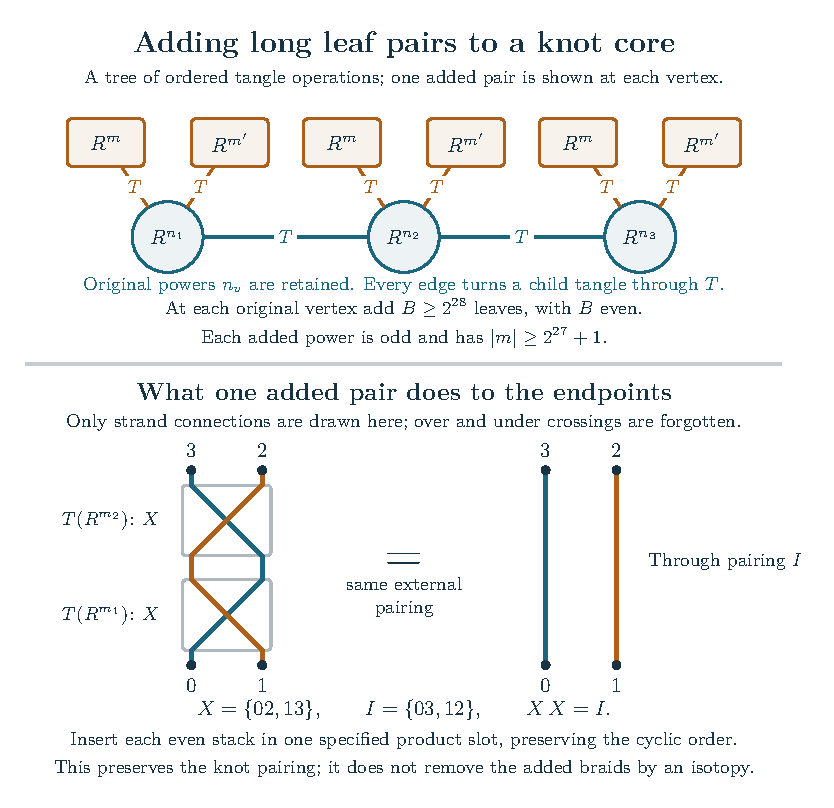
\includegraphics[width=.88\linewidth,height=.65\textheight,keepaspectratio]{../book/figures/directed-tree-volume.pdf}
\caption{Adding terminal pieces in pairs. The upper diagram records the tangle operations; only one of the required pairs is shown at each original vertex. Below, following the strands through two odd pieces gives two through connections. The endpoint pairing is preserved, while the knot type can change.}
\label{fig:directed-core-extension}
\end{figure}

\begin{corollary}\label{cor:directed-core-extension}
The resulting knot has a hyperbolic complement and satisfies
\eqref{eq:directed-volume} and \eqref{eq:directed-profile}.
The initial tree, all original powers, all inserted pieces and
their powers are fixed before $N$ tends to infinity.
\end{corollary}

This construction preserves the short-twist pieces and their endpoint
connections; it generally changes the knot. The corollary therefore
constructs a larger family of knots satisfying the volume identity.
It does not assert the identity for every unchanged short-twist
diagram from which the construction starts.

\section{A finite criterion beyond the simple bounds}

The choice of final vertex matters even with equal $c_v$. Consider
a star with $30{,}000{,}001$ terminal vertices. Give the center power
$2$ and each terminal vertex power $2^{60}+1$, and evaluate the
center last. The original strand calculation gives one knot.
For the center, exact rational bounds imply
\[
                   \frac{\beta_o}{\eta_o/2}<0.9.
\]
Its value of $\beta_o$ exceeds
$k_0(1-\cos r_0)$, so it cannot satisfy an outgoing condition for
any positive $c_o$. It need not do so because it is evaluated last.
The terminal vertices satisfy all their own conditions.

The summed test also fails for this example:
\[
 \sum_v\frac{d_v}{d_v^2+n_v^2}
 \ge\frac{30{,}000{,}001}{30{,}000{,}001^2+4}>2^{-25}.
\]
The example shows a precise benefit of the directed criterion.
Its size is deliberately conservative; no claim of a smallest such
example is needed. Appendix~\ref{app:directed-circle-messages}
gives the endpoint pairing calculation and the exact rational
inequalities, with a single reproduction command in
Chapter~\ref{ch:reproduction}.
